\documentclass[ 11pt,%
				a4paper,% 
				oneside,% 
				headinclude,% 
				footinclude = true,% 
				cleardoublepage = empty,% 
				reqno]{scrbook}






%!TEX root = Probability_Notes.tex

% fonts
\usepackage[proportional,scaled=1.064]{erewhon}
\usepackage[erewhon,vvarbb,bigdelims]{newtxmath}
\renewcommand*\oldstylenums[1]{\textosf{#1}}
\usepackage[T1]{fontenc}
\usepackage[utf8]{inputenc}
\usepackage{anyfontsize}
\usepackage{chancery}
\usepackage{calrsfs}
\usepackage{mathrsfs}
\usepackage{relsize} % large math
\usepackage[english]{babel}
\usepackage[math]{blindtext}  

% line spacing
\usepackage{setspace}


%header
\usepackage{titlesec}

\usepackage{blindtext}
\usepackage{color}


% show labels

\usepackage[notref]{showkeys}
\setlength{\fboxrule}{0pt}
\setlength{\fboxsep}{0pt}
\renewcommand*{\showkeyslabelformat}[1]{%
   \framebox{\fbox{\vbox{\hsize=1cm\normalfont\small\url{#1}\par}}}}
% \usepackage[right]{showlabels}


% referencing
\usepackage{nameref}


% cite, link color
\usepackage[colorlinks=true,
			linkcolor=red!60!black, 
			citecolor=red!20!black]{hyperref}
\usepackage[capitalise]{cleveref}


%box
\usepackage{longfbox}


%%fonts


%appendix theorem number
\usepackage{appendix}
\usepackage{apptools}
\AtAppendix{\counterwithin{definition}{chapter}}


%quote
\usepackage[autostyle]{csquotes} 

%stackoverflow solution

% \usepackage[capitalise]{cleveref}
% \makeatletter
% \if@cref@capitalise
% \crefname{theorem}{TheoUpperCase}{TheoUppercasesS}
% \else
% \crefname{theorem}{theoLowercase}{theoLowercaseS}
% \fi
% \makeatother
% \Crefname{theorem}{TheoUpperCase}{TheoUppercasesS}

\Crefname{definition}{\bfseries Definition}{}
\Crefname{theorem}{Theorem}{}
\Crefname{example}{Example}{}
\Crefname{remark}{Remark}{}
\Crefname{axioms}{Axioms}{}



% some packages I added, forgot why?

\usepackage{lipsum,multicol}

% for custom margin
\usepackage{changepage}
\usepackage{ragged2e}
\usepackage{amsmath, amsthm, amsfonts, amssymb,thmtools}
\usepackage{booktabs}
\usepackage{multirow}
\usepackage{graphicx}
\usepackage{adjustbox}
\usepackage{dsfont}
\usepackage{ifsym}
\usepackage{fancyhdr}
% \usepackage{anysize}
%\usepackage{makeidx}
% \usepackage{twoopt}
\usepackage{mleftright}
\usepackage{mathtools}
\usepackage{ifthen}
\usepackage{xcolor}
\usepackage{xspace}
\usepackage{chngcntr}
\usepackage{mdframed}
\usepackage{sidenotes} 
\usepackage{mwe} 
\usepackage{accents}
\usepackage{paralist}
\usepackage[shortlabels]{enumitem}
\usepackage{dictsym}
\usepackage{textgreek}
\usepackage{etoolbox} 
\usepackage{empheq}
\usepackage{url}
\usepackage{array}
\usepackage{type1ec}
\usepackage{blkarray}
\usepackage[makeroom]{cancel}
\usepackage{hhline}
\usepackage[percent]{overpic}

% Don't use mparhack.
\usepackage{marginfix}
\usepackage[color]{changebar}
\usepackage{marginnote}
\usepackage{todonotes}
\usepackage{parskip}
%\usepackage{refcheck}
\usepackage{ellipsis}




%symbols
\usepackage{textcomp}
\usepackage{manfnt}
\usepackage{physics}
\usepackage{MnSymbol}
\usepackage{pifont}
\usepackage{yfonts}
\usepackage{float}
\usepackage{bclogo}

%............


% for caption
\usepackage[format=plain,
            labelfont={it},
            textfont=it]{caption}


% footnote configuration
\usepackage[hang,flushmargin]{footmisc}


% tikz
\usepackage{tkz-berge}
\usepackage{pgf, tikz}
\usepackage{pgfplots}
\usepgflibrary{fpu}
\usetikzlibrary{shapes, matrix, cd, decorations,arrows,calc,arrows.meta,fit,positioning, decorations.markings, snakes, math, fadings, intersections}

% pstricks failed
\usepackage{pst-plot,pst-func,pstricks}
\usepackage{pst-eucl}
\usepackage{pstricks-add}

% bib
\usepackage[sort&compress, round ,comma,authoryear]{natbib}

\usepackage{venndiagram}









%%%%%%%%%%%%%%%%%%%%%%%%%%%%%%%%%







%!TEX root = Probability_Notes.tex

%colors
\definecolor{napiergreen}{rgb}{0.16, 0.5, 0.0}
\definecolor{gray75}{gray}{0.75}

\definecolor{gainsboro}{rgb}{0.86, 0.86, 0.86}
\definecolor{linen}{rgb}{0.98, 0.94, 0.9}
\definecolor{moccasin}{rgb}{0.98, 0.92, 0.84}
\definecolor{oldlavender}{rgb}{0.47, 0.41, 0.47}
\definecolor{palecerulean}{rgb}{0.61, 0.77, 0.89}
\definecolor{gold}{rgb}{0.85,0.65,0}
\definecolor{maroon}{rgb}{0.5, 0.0, 0.0}


\newcommand{\cthm}[1]{\textcolor{red!30!black!}{#1}}
\newcommand{\cdefn}[1]{\textcolor{darkblue!30!black!}{#1}}
\newcommand{\cexm}[1]{\textcolor{darkgoldenrod!60!black}{#1}}
\newcommand{\crem}[1]{\textcolor{glaucous!30!black!}{#1}}


%geogebra tikz
\pgfplotsset{compat=1.15}

% page area 
\areaset[current]{440pt}{800pt} 

% % marginwidth
\setlength{\marginparwidth}{5em}%
\setlength{\marginparsep}{1.5em}%

% line spacings...
\setstretch{1}
\setlength{\parskip}{\baselineskip}%

% image path
\graphicspath{{image/}} 


%box eqn
\newcommand{\boxalign}[2][0.97\textwidth]{
  \par\noindent\tikzstyle{mybox} = [draw=black,inner sep=6pt]
  \begin{center}\begin{tikzpicture}
   \node [mybox] (box){%
    \begin{minipage}{#1}{\vspace{-5mm}#2}\end{minipage}
   };
  \end{tikzpicture}\end{center}
}

% % marginnote
% \marginskip{0em}
\newcommand{\marginbreak}[1]{\renewcommand*{\marginnotevadjust}{#1}}




%%showkeys

% \renewcommand*{\showkeyslabelformat}[1]{%
%    \fbox{\vbox{\hsize=1cm\normalfont\small\url{#1}\par}}}





% color for the changebar package
\cbcolor{blue}


% some color shortcuts



% format titles

\newcommand{\hsp}{\hspace{20pt}}
\titleformat{\chapter}{\Huge\bfseries}{\thechapter\hsp\textcolor{gray75}{|}\hsp}{0pt}{\Huge\bfseries}
\titlespacing*{\chapter}{0pt}{-30pt}{40pt}

% \titleformat{\chapter}{\Large\bfseries}{\thechapter}{1em}{}
% \titlespacing*{\chapter}{0pt}{15pt}{4pt}

\setcounter{secnumdepth}{3}

\titleformat{\section}{\Large\bfseries}{\thesection}{1em}{}
\titlespacing*{\section}{0pt}{15pt}{4pt}


\titleformat{\subsection}{\color{gray!30!black}\large\bfseries}{\thesubsection}{1em}{}[]
\titlespacing*{\subsection}{0pt}{12pt}{5pt}
% this alters "before" spacing (the second length argument) to 0

\titleformat{\subsubsection}{\color{gray!60!black}\itshape\bfseries}{\thesubsubsection}{1em}{}[]
\titlespacing*{\subsubsection}{0pt}{10pt}{0pt}




% Custom font

% custom font nadia
\newenvironment{myfont}{\fontfamily{qag}\selectfont}{\par}
\DeclareTextFontCommand{\textmyfont}{\myfont}

% custom font theorem
\newenvironment{theofont}{\fontfamily{qzc}\selectfont}{\par}
\DeclareTextFontCommand{\ttheofont}{\theofont}



% dictum
\setkomafont{dictumtext}{\itshape}
\setkomafont{dictumauthor}{\normalfont}
\renewcommand*\dictumwidth{0.66\linewidth}
\renewcommand*\dictumauthorformat[1]{\smallskip

--- #1\vspace{3em}}
\renewcommand*\dictumrule{}
%\renewcommand{\raggeddictumtext}{\RaggedLeft}
\renewcommand{\raggeddictumtext}{\raggedleft}

%
\newcommand{\dictumold}{}  
\let\dictumold\dictum  
\renewcommand{\dictum}{\vspace{1em}\dictumold} 

% marginfont
\renewcommand*{\marginfont}{\slshape\footnotesize}



% emphasize color
\renewcommand{\emph}[1]{%
  {\textcolor{green!35!black}{\itshape#1}}%
}


% parskip
\parskip 1.3ex



% remove chapter number and section number

\newcommand{\mychapter}[2]{
    \setcounter{chapter}{#1}
    \chapter*{#2}
    \addcontentsline{toc}{chapter}{#2}
}

\newcommand{\mysection}[2]{
    \setcounter{section}{#1}
    \section*{#2}
}


%toc
\setcounter{tocdepth}{3}




%!TEX root = Probability_Notes.tex

% side rules for theorem environment



%Theorem, Corollary, Proposition, Lemma

%Defintion, Assumptions

\definecolor{darkblue}{rgb}{0.0, 0.0, 0.55}
\newtheoremstyle{defnstyle}
  {} % Space above
  {} % Space below
  {} % Body font
  {} % Indent amount
  {{\hspace{-.2cm} \color{darkblue!40!black}\ding{118}}~\itshape\bfseries\color{darkblue!40!black}} %  head font
  {.} % Punctuation after  head
  {.5em} % Space after head
  {} %  head spec (can be left empty, meaning `normal')
\theoremstyle{defnstyle} 
\newtheorem{definition}{Definition}[chapter] 
\newtheorem{assumptions}[definition]{Assumption} 
\newtheorem{axioms}[definition]{Axioms} 



\newtheoremstyle{theostyle}
  {} % Space above
  {} % Space below
  {} % Body font
  {} % Indent amount
  {{\hspace{-.2cm} \color{red!30!black!}\ding{69}}~\itshape\bfseries\color{red!30!black!}} % Theorem head font
  {.} % Punctuation after theorem head
  {.5em} % Space after theorem head
  {} % Theorem head spec (can be left empty, meaning `normal')
\theoremstyle{theostyle} 
\newtheorem{theorem}[definition]{Theorem}%%% changed
\newtheorem*{theorem*}{Theorem} %%% changed
\newtheorem{corollary}[definition]{Corollary} %%% changed
\newtheorem{proposition}[definition]{Proposition} %%% changed
\newtheorem{lemma}[definition]{Lemma} %% chaged
% \newtheorem{hyp}[theorem]{Hypothesis} %%% changed

%--------------------------------



% Examples,
\definecolor{darkgoldenrod}{rgb}{0.72, 0.53, 0.04}
\newtheoremstyle{exmstyle}
  {} % Space above
  {} % Space below
  {} % Body font
  {} % Indent amount
  {{\hspace{-.1cm}\color{darkgoldenrod!60!black} \ding{168}}~\bfseries\color{darkgoldenrod!60!black}} %  head font
  {.} % Punctuation after  head
  {.5em} % Space after head
  {} %  head spec (can be left empty, meaning `normal')
\theoremstyle{exmstyle}
\newtheorem{example}[definition]{Example} %%% changed

% Remark, Remarks,
  \definecolor{glaucous}{rgb}{0.38, 0.51, 0.71}
\newtheoremstyle{remstyle}
  {} % Space above
  {} % Space below
  {} % Body font
  {} % Indent amount
  {{\hspace{-.55cm}  \color{glaucous!30!black} \ding{46}}~\bfseries\color{glaucous!30!black}} %  head font
  {.} % Punctuation after  head
  {.5em} % Space after head
  {} %  head spec (can be left empty, meaning `normal')
\theoremstyle{remstyle}
\newtheorem{remark}[definition]{Remark} %%% changed
\newtheorem{remarks}[definition]{Remarks}%%% changed



% \newtheorem*{theorem*}{Theorem}
\newtheorem*{claim}{Claim}

%notation

\newtheoremstyle{notation}
  {} % Space above
  {} % Space below
  {} % Body font
  {} % Indent amount
  {{\hspace{-.75cm}  \color{gray!10!black!} \lhdbend}~\bfseries\color{gray!80!black!}} %  head font
  {:} % Punctuation after  head
  {.5em} % Space after head
  {} %  head spec (can be left empty, meaning `normal')
\theoremstyle{notation}
\newtheorem*{notation}{{Notes on notations}}


\AtBeginEnvironment{theorem}{\begin{minipage}{\textwidth}\noindent\vspace*{.2cm}}
\AtEndEnvironment{theorem}{\end{minipage}\vspace*{0cm}\flushright \color{red!30!black!}\textminus\textminus\textminus \ding{69}  }

\AtBeginEnvironment{lemma}{\begin{minipage}{\textwidth}\vspace*{.3cm}}
\AtEndEnvironment{lemma}{\end{minipage}\vspace*{.3cm}}

\AtBeginEnvironment{definition}{\begin{minipage}{\textwidth}\noindent\vspace*{.2cm}}
\AtEndEnvironment{definition}{\end{minipage}\vspace*{0cm}\flushright \color{darkblue!40!black}\textminus\textminus\textminus \ding{118} }




% \AtBeginEnvironment{assumption_n}{\begin{minipage}{\textwidth}\vspace*{.3cm}}
% \AtEndEnvironment{assumption_n}{\vspace*{-27pt}\flushright{\trpslash}\end{minipage}\vspace*{.3cm}}

% \AtBeginEnvironment{assumption}{\begin{minipage}{\textwidth}\vspace*{.3cm}}
% \AtEndEnvironment{assumption}{\vspace*{-27pt}\flushright{\trpslash}\end{minipage}\vspace*{.3cm}}

% \AtBeginEnvironment{example}{\vspace*{.3cm}}
\AtEndEnvironment{example}{\color{darkgoldenrod!60!black!} \flushright{\textit{(...end of example!)}}}


%% numbering of theorems



% changing the numbering of theorem and equations
% \numberwithin{section}{chapter}
% \numberwithin{equation}{chapter}
% \counterwithin{equation}{chapter}


% color brackets
\makeatletter
\newcount\bracketnum
\newcommand\makecolorlist[1]{%
    \bracketnum0\relax
    \makecolorlist@#1,.%
    \bracketnum0\relax
}
\def\makecolorlist@#1,{%
    \advance\bracketnum1\relax
    \expandafter\def\csname bracketcolor\the\bracketnum\endcsname{\color{#1}}%
    \@ifnextchar.{\@gobble}{\makecolorlist@}%
}
\let\oldleft\left
\let\oldright\right
\def\left#1{%
    \global\advance\bracketnum1\relax 
    \colorlet{temp}{.}%
    \csname bracketcolor\the\bracketnum\endcsname
    \oldleft#1%
    \color{temp}%
}
\def\right#1{%
    \colorlet{temp}{.}%
    \csname bracketcolor\the\bracketnum\endcsname
    \oldright#1%
    \global\advance\bracketnum-1\relax
    \color{temp}%
}
\makeatother


\makecolorlist{black,blue,red}




% 2 independent signs

% indep one
\newcommand{\indep}{\raisebox{0.05em}{\,\rotatebox[origin=c]{90}{\mbox{\Large$\models$}} \,} }
\newcommand{\indepG}{{\indep}_{\mbox{\tiny$\mkern-18mu\mathcal{G}$}}}

% independent one
\newcommand\independent{\protect\mathpalette{\protect\independenT}{\mbox{\Large$\perp$}}}
\def\independenT#1#2{\mathrel{\rlap{$#1#2$}\mkern2mu{#1#2}}}

\newcommand{\independentG}{{\independent}_{\mbox{\scriptsize$\mkern-6mu\mathcal{G}$}}}

% argmin, argmax
\DeclareMathOperator*{\argmax}{arg\,max}
\DeclareMathOperator*{\argmin}{arg\,min}


% combination notation

\newcommand\Myperm[2][^n]{\prescript{#1\mkern-2.5mu}{}P_{#2}}
\newcommand\Mycomb[2][^n]{\prescript{#1\mkern-0.5mu}{}C_{#2}}




% distributed as
\makeatletter
\newcommand{\distas}[1]{\mathbin{\overset{#1}{\kern\z@\sim}}}%
\newsavebox{\mybox}\newsavebox{\mysim}
\newcommand{\distras}[1]{%
  \savebox{\mybox}{\hbox{\kern3pt$\scriptstyle#1$\kern3pt}}%
  \savebox{\mysim}{\hbox{$\sim$}}%
  \mathbin{\overset{#1}{\kern\z@\resizebox{\wd\mybox}{\ht\mysim}{$\sim$}}}%
}
\makeatother


% tikz

\pgfarrowsdeclare{my to}{my to}
{
  \pgfarrowsleftextend{-2\pgflinewidth}
  \pgfarrowsrightextend{\pgflinewidth}
}
{
  \pgfsetlinewidth{1.4\pgflinewidth}
  \pgfsetdash{}{0pt}
  \pgfsetroundcap
  \pgfsetroundjoin
  \pgfpathmoveto{\pgfpoint{-5.5\pgflinewidth}{7.5\pgflinewidth}}
  \pgfpathcurveto
  {\pgfpoint{-4.0\pgflinewidth}{0.1\pgflinewidth}}
  {\pgfpoint{0pt}{0.25\pgflinewidth}}
  {\pgfpoint{0.75\pgflinewidth}{0pt}}
  \pgfpathcurveto
  {\pgfpoint{0pt}{-0.25\pgflinewidth}}
  {\pgfpoint{-4.0\pgflinewidth}{-0.1\pgflinewidth}}
  {\pgfpoint{-5.5\pgflinewidth}{-7.5\pgflinewidth}}
  \pgfusepathqstroke
}


\newcommand{\asymcloud}[2][.1]{%
\begin{scope}[#2]
\pgftransformscale{#1}%    
\pgfpathmoveto{\pgfpoint{261 pt}{115 pt}} 
  \pgfpathcurveto{\pgfqpoint{70 pt}{107 pt}}
                 {\pgfqpoint{137 pt}{291 pt}}
                 {\pgfqpoint{260 pt}{273 pt}} 
  \pgfpathcurveto{\pgfqpoint{78 pt}{382 pt}}
                 {\pgfqpoint{381 pt}{445 pt}}
                 {\pgfqpoint{412 pt}{410 pt}}
  \pgfpathcurveto{\pgfqpoint{577 pt}{587 pt}}
                 {\pgfqpoint{698 pt}{488 pt}}
                 {\pgfqpoint{685 pt}{366 pt}}
  \pgfpathcurveto{\pgfqpoint{840 pt}{192 pt}}
                 {\pgfqpoint{610 pt}{157 pt}}
                 {\pgfqpoint{610 pt}{157 pt}}
  \pgfpathcurveto{\pgfqpoint{531 pt}{39 pt}}
                 {\pgfqpoint{298 pt}{51 pt}}
                 {\pgfqpoint{261 pt}{115 pt}}
\pgfusepath{fill,stroke}         
\end{scope}}  


% \tikzset{-{{To}[length=1.3mm,line width=1.3pt]}, auto, 
%     state/.style ={circle, draw, minimum width = 0.1 cm, scale=0.9},
%     point/.style = {circle, draw, inner sep=0.02cm,fill,node contents={}},
%     bidirected/.style={Latex-Latex,dashed},
%     hidden/.style={dashed}
%     }

\newcommand{\tikzl}[1]{{\begin{tikzpicture}#1\end{tikzpicture}}}
\newcommand{\tikzm}[1]{\footnotesize{\begin{tikzpicture}#1\end{tikzpicture}}}


% qed symbol
\renewcommand{\qedsymbol}{\rule{0.4em}{0.4em}}


\newcommand{\trpslash}{\textcolor{green!35!black}{\textbackslash\hspace{-.15cm}\textbackslash\hspace{-.15cm}\textbackslash   }}

\newcommand{\lgreen}{green!15!white}


%writing hand
\newcommand\Writinghand{{\fontfamily{mvs}\fontencoding{U}\selectfont\char98}}



%% argmin
\DeclareMathOperator*{\argminNS}{argmin}  
\DeclareMathOperator*{\argmaxNS}{argmin}  



%align space

\newcommand{\zerodisplayskips}{%
  \setlength{\abovedisplayskip}{-10pt}%
  \setlength{\belowdisplayskip}{8pt}%
  \setlength{\abovedisplayshortskip}{0pt}%
  \setlength{\belowdisplayshortskip}{0pt}}
\appto{\normalsize}{\zerodisplayskips}
\appto{\small}{\zerodisplayskips}
\appto{\footnotesize}{\zerodisplayskips}

% Hide subsections from TOC.
% \setcounter{tocdepth}{1}

\raggedbottom
\allowbreak
\sloppy






\begin{document}
\pagenumbering{roman}


%% title page
\begin{titlepage}
    \vspace*{9em}{\centering\Huge\usefont{T1}{qzc}{m}{it}
Basics of Probability\par}
\vspace{1em}
{\hfill\itshape Very short introduction}
\clearpage
    \vspace*{\fill}\hfill   \parbox{.4\textwidth}{
    \raggedleft
\scriptsize These notes are a quick and dirty introduction to probability theory!  \emph{Tanvir!}
}
\end{titlepage}
%%



\begingroup
\hypersetup{linkcolor=gainsboro!60!black}
\tableofcontents
\endgroup


\frontmatter
\pagenumbering{arabic}


% \setcounter{chapter}{3}
\mainmatter



\chapter{Probability Space}

	The object of probability theory is to describe and investigate mathematical models of random phenomena, primarily from a theoretical point of view. Closely related to probability theory is statistics, which is concerned with creating principles, methods, and criteria in order to treat data pertaining to such (random) phenomena or data from experiments and other observations of the real world, by using, for example, the theories and knowledge available from the theory of probability.

	Probability theory thus aim at describing \emph{random experiments}. We will shortly explain what do we mean by random experiments. But before that you should know the basis of probability theory is the \emph{probability space} which is written $(\Omega, \mathcal{F}, P)$. You really need to understand each of the three things that we have written here. First let us give the names of these three elements. $\Omega$ is what we call \emph{sample space}, $\mathcal{F}$ is what we call \emph{event space} (another imprtant name $\sigma$-algebra) and $P$ is our dearest \emph{probability function} (another important name probability measure). Each of the three plays significant role in understanding probability. You might be wondering, why this complication? why not simply calculate probabilities from counting? Well welcome to mathematics, because in mathematics we hate inconsistencies. So we will \emph{define} probability in a way so that we get meaningful probabilities.  OK Lets start. Since everything starts from experiment. First we explain what is an experiment.

	\begin{definition}[Experiment, Random Experiment and Events]~\label{def:re}
		An \emph{experiment} is any process, real or hypothetical, in which \emph{all possible outcomes} can be identified \emph{ahead of time}. We call an experiment \emph{random experiment} when we do not know which outcomes will appear. An \emph{event} is a well-defined \emph{set} of possible outcomes of the experiment.
	\end{definition}

	\begin{example}[Toissing a coin]~\label{ex:tosscoin}
		If we toss a coin we know the outcomes can be head or tail. So we know all possible outcomes, but we do not beforehand which will come when we toss a particular coin. So tossing a coin is the random experiment.
	\end{example}


	\begin{example}[Throwing a dice]~\label{ex:throwdice}
		Similarly when we trow a dice we know that any number between 1 to 6 might appear, but before throwing it we do not know which one will exactly come. So throwing a dice is the random experiment.
	\end{example}

	\begin{example}[Tossing multiple coins]~\label{ex:tossmulticoin}
		A slightly complex example is when we trow toss more than one coins together. The experiment in this case is tossing more than one coins. For example, think about tossing three coins, we know all the outcomes, that is we know that our \emph{realization} could be

		\begin{align*}
		(H, H, H) \text{ or } (H, H, T), \text{ or } (H, T, H), \text{ or } \\
		(H, T, T), \text{ or } (T, H, H), \text{ or } (T, H, T), \text{ or } \\
		(T, T, H), \text{ or } (T, T, T), \text{ or } (H, H, H)
		\end{align*}
	\end{example}

		
	\section{Sample space}
		Now that we have defined random experiment (again random means, beforehand we do not know which outocme will appear), we can define \emph{Sample Space}. So sample space is a \emph{set} (you should know some set theory from the basic math course!). It is the set of all possible outcomes. We will denote the sample space with $\Omega$.

		\begin{example}[Continuation of \cref{ex:tosscoin}]
		When we toss a coin, the sample is the set $\Omega = \{H, T\}$
		\end{example}


		\begin{example}[Continuation of \cref{ex:throwdice}]
		When we throw a dice the sample space is $\Omega = \{1,2,3,4,5,6\}$
			
		\end{example}


		\begin{example}[Continuation of ]~\label{ex:tossmulticoin2}
		When we throw three coins together then we have a big sample space of 8 possible outcomes, 

		\begin{align*}
				\Omega = \left\{ (HHH) , (THH)  (HTH)  (HHT) \\ (HTT) , (THT) ,
				(TTH) , (TTT)  \right. \}
		\end{align*}

		We will use these example a lot, so let us write this example with easy notation, let us denote 

		\begin{align*}
		\omega_{1}:  \mathrm{HHH}, \quad \omega_{2}:  \mathrm{THH}, \quad \omega_{3}:  \mathrm{HTH} \quad \omega_{4}: \mathrm{HHT} \\
		 \omega_{5}:  \mathrm{HTT}, \quad  \omega_{6}:  \mathrm{THT} \quad \omega_{7}:  \mathrm{TTH}, \quad \omega_{8}:  \mathrm{TTT}
		\end{align*}

		Now we can write the same sample space as 

		\begin{align*}
			\Omega =\left\{\omega_{1}, \omega_{2}, \omega_{3}, \omega_{4}, \omega_{5}, \omega_{6}, \omega_{7}, \omega_{8} \right\},
		\end{align*}

		which looks much better. 
		\end{example}


	\section{Event space}
		
		Now let us talk about event space, the idea about event space is this is where we would like to assign probabilities. This will become clear soon, but let us define first what is an event.

		\begin{definition}[Event]
		An event is a subset of the sample space. And often we denote this with the letters $A$. $B$, $C$, etc.
		\end{definition}

		So if the sample space is the big set $\Omega$, an event is just a subset. Note it can be any subset as long as it is a subset of $\Omega$.

		\begin{example}[]
			If we want to define an event in \cref{ex:tossmulticoin2}, we can simply take any subset $A \subset \Omega$, where $A = \{\omega_1, \omega_8\}$
		\end{example}

		The last example just took a subset which may not habe any meaning. This is a valid event. But in probability theory we often define event to be a meaningful set. So let us define some events.

		\begin{example}[Continuation of \cref{ex:tossmulticoin2}]

		If $A$ is an event that \emph{at least} one head is obtained in the 3 tosses; then 

		\begin{align*}
		A=\left\{\omega_{1}, \omega_{2}, \omega_{3}, \omega_{4}, \omega_{5}, \omega_{6}, \omega_{7}\right\}
		\end{align*}


		If $B$ is an event that \emph{one head is obtained on the second toss}; 

		\begin{align*}
			B=\left\{\omega_{1}, \omega_{2}, \omega_{4}, \omega_{6}\right\}
		\end{align*}


		let $C$ be the event that \emph{one tail is obtained on the third toss}, so

		\begin{align*}
			C=\left\{\omega_{4}, \omega_{5}, \omega_{6}, \omega_{8}\right\} 
		\end{align*}

		finally let $D$ be the event that \emph{no heads are obtained}. Accordingly,

		\begin{align*}
			D=\left\{\omega_{8}\right\}
		\end{align*}
			
		\end{example}

		So event is simply a subset. What about \emph{event space}. Event space is the set of \emph{all (well defined) events}. So simply we should take all ``nice'' events and put them in a set, so that we get a \emph{set of events} and that set is what we call the event space. Note, the events itself are sets, so when we again make another set with events we have a \emph{set of sets}. For example, power set is the set of all possible subsets. The problem is how do we define ``nice'' or ``well behaved'' that we have written in the definition. We will not into the details of this concept. You will learn it in detail in the Statistical Theory course. But we get the nice set of subsets. When we have a finite sample space, for all of our example, \cref{ex:tosscoin,ex:tossmulticoin,ex:throwdice} we have finite $\Omega$, the nice sets or the event space is just simply the power set. Let us look at some example

		\begin{example}[Power set as Event space]
		For example we can take $\Omega = \{\omega_1, \omega_2, \omega_3 \}$. So this is our sample. Now for this set $\Omega$, what is the power set of this set? It is the set all possible outcomes

		\begin{align*}
			\mathscr{P}(\Omega) =\{ & \emptyset, \\
								 & \{ \omega_1 \}, \{ \omega_2 \}, \{ \omega_3 \}, \\
								 & \{ \omega_1, \omega_2 \}, \{ \omega_2, \omega_3 \}, \{ \omega_1, \omega_3 \}\\
								 & \{ \omega_1. \omega_2, \omega_3\} \}
		\end{align*}


		In this case the event space which is the \emph{set of nice subsets} of $\Omega$ is the power set, which is the set of all outcomes, so the event space is same 

		\begin{align*}
			\mathcal{F} =\{ & \emptyset, \\
							 & \{ \omega_1 \}, \{ \omega_2 \}, \{ \omega_3 \}, \\
							 & \{ \omega_1, \omega_2 \}, \{ \omega_2, \omega_3 \}, \{ \omega_1, \omega_3 \}\\
							 & \{ \omega_1. \omega_2, \omega_3\} \}
		\end{align*}
			
		\end{example}


		Again we emphasize it, event space is a particular set of subsets of $\Omega$. We have not given you the definition of event space, you do not need it for now. Just remember its a special set of subsets. It may or may note be the power set. In the case of finite sample space, when $\Omega$ is finite, power set satisfies the definition of the event space, so that is why power set is the event space. For infinite cases, meaning $\Omega$ is infinite. for example, when $\Omega = \mathbb{R}$, power set IS NOT an event space, we need a special set of sets then. 

		You can ask why do we need to define  event space, the short answer is we would like to calculate probabilities on events of the sample space. For example if $A = \{ \omega_1, \omega_2, \omega_3\}$ is an event of $\Omega$, we would like to calculate the probability of happening $\Omega$, or in other words $P(A)$. But what is probability $P$? This is what we will define in the next section. 

		\section{Probability}

			The mathematical definition of probability will satisfy three \emph{axioms}. You can think about axioms as some kind of grand rules, that we just take it as some rules that we will assume will always hold. Its actually very much like definition. In probability theory mathematicians came up with three axioms, or rules of probability and then they said for $P$ to be a probability on any set $A$, following three rules must hold

			\begin{axioms}[Axioms of Probability]~\label{axiom:Kolmogorov}
				\begin{itemize}
					\item[]
					\item[a1.] For every event $A \subset \Omega$ $\operatorname{P}(A) \geq 0$.

					\item[a2.] $\operatorname{P}(\Omega)=1$

					\item[a3.] For every infinite sequence of disjoint events $A_{1}, A_{2}, \ldots,$

					\begin{align*}
						\operatorname{P}\left(\bigcup_{i=1}^{\infty} A_{i}\right)=\sum_{i=1}^{\infty} \operatorname{P}\left(A_{i}\right)
					\end{align*}

				\end{itemize}
			\end{axioms}


			Now that we have the axioms, we can define \emph{probability},

			\begin{definition}[Probability]
				\emph{A probability measure}, or simply a \emph{probability}, on a sample space $\Omega$ is a set function, such that $\operatorname{P}(A)$ for all events $A$ will satisfy \cref{axiom:Kolmogorov}.
			\end{definition}

			So any set function as long as it satisfies the axioms will be a probability function. Let us quickly mention some of the rules of probability. You should try to prove this, if not now at least remember this

			\begin{theorem}
				For any set $A\subset\Omega$, and $B \subset \Omega$

				\begin{itemize}

					\item $\operatorname{P}(\emptyset)=0$.
					\item For every finite sequence of $n$ disjoint events $A_{1} \ldots \ldots, A_{n}$

						\begin{align*}
							\operatorname{P}\left(\bigcup_{i=1}^{n} A_{i}\right)=\sum_{i=1}^{n} \operatorname{P}\left(A_{i}\right)
						\end{align*}

					\item $\operatorname{P}\left(A^{c}\right)=1-\operatorname{P}(A)$

					\item  If $A \subset B, \text { then } \operatorname{P}(A) \leq \operatorname{P}(B)$

					\item  $0 \leq \operatorname{P}(A) \leq 1$

					\item For $A$ and $B$

						\begin{align*}
							\operatorname{P}\left(A \cap B^{c}\right)=\operatorname{P}(A)-\operatorname{P}(A \cap B)
						\end{align*}
						

					\item For $A$ and $B$
						
						\begin{align*}
								\operatorname{P}(A \cup B)=\operatorname{P}(A)+\operatorname{P}(B)-\operatorname{P}(A \cap B)
						\end{align*}
					
					
						
						
				\end{itemize}
			\end{theorem}


	So we have already explained the three elements of the probability space that $\Omega, \mathcal{F}, P$, $\Omega$ is the sample space which is the set of all possible outcomes, $\mathcal{F}$ is the \emph{set of nice subsets of} $\Omega$, when $\Omega$ is a finite set, then $\mathcal{F}$ is a power set, but if  $\Omega$ is any infinite set. e.g., $\Omega = \mathbb{R}$. It tuns out we cannot take power set as a event space, because we cannot consistently assign probabilities. So we have to choose in general. You do not need more details on this now. Finally $P$ is any \emph{set} function that will satisfy certain axioms, in particular \cref{axiom:Kolmogorov}. Let us see one complete example,

\begin{example}[Throwing a dice example]

Recall the dice example, our sample space was 

\begin{align*}
\Omega=\{1,2,3,4,5,6\}
\end{align*}

You can think about the event space, which is the power set in this case. Now we need to come up with an idea how we can assign probabilities for each subset $A$ of $\Omega=\{1,2,3,4,5,6\}$. Let us do the following, let $\operatorname{P}(A)$ be the number of elements of $A$ divided by $6$. Then it is easy to see that this satisfies the first two axioms. There are only finitely many distinct collections of nonempty disjoint events. It is not difficult to see that the third axiom is also satisfied by this example.


There are also ways to assign probabilities. For example, if we believe that the die is loaded, we might believe that some sides have different probabilities of turning up. To be specific, suppose that we belicve that 6 is twice as likely to come up as each of the other five sides. We could set $p_{j}=1 / 7$ for $i=1,2,3,4,5$ and $p_{6}=2 / 7 .$ Then, for each event $A,$ define $\operatorname{P}(A)$ to be the sum of all $p_{i}$ such that $i \in A .$ For example, if $A=\{1,3,5\},$ then $\operatorname{P}(A)=p_{1}+p_{3}+p_{5}=3 / 7$ It is not difficult to check that this also satisfies all three axioms.

So the idea is, if I design/know how will I calculate the probabilities, then if you give me any subset $A$ of $\Omega$ (that is part of the nice set of subsets), I can calculate the probabilities of that set. 
	
\end{example}

\chapter{Conditional Probability}


\section{Conditional Probability: Definition and exmaples}

\begin{figure}[H]
\begin{center}
	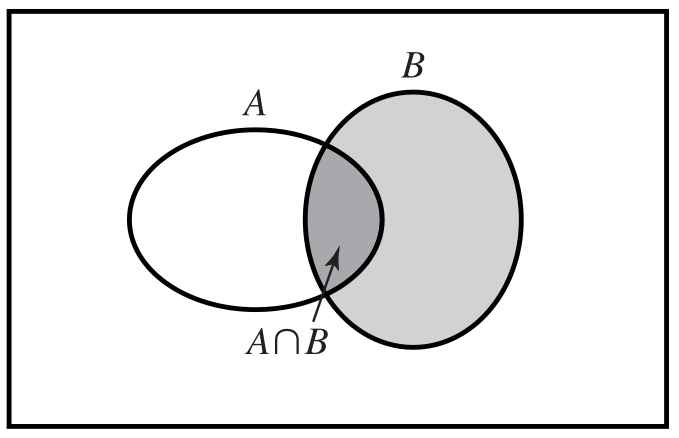
\includegraphics[scale = .4]{images/condProb.png}
\end{center}
	
\end{figure}

\begin{definition}[Conditional Probability]
Suppose that we learn that an event $B$ has occurred and that we wish to compute the probability of another event $A$ taking into account that we know that $B$ has occurred. The new probability of $A$ is called the conditional probability of the event A given that the event $B$ has occurred and is denoted $\operatorname{P}(A | B)$
If $\operatorname{P}(B)>0,$ we compute this probability as

\begin{align}~\label{eq:conp}
	\operatorname{P}(A | B)=\frac{\operatorname{P}(A \cap B)}{\operatorname{P}(B)}
\end{align}


The conditional probability $\operatorname{P}(A | B)$ is not defined if $\operatorname{P}(B)=0$
\end{definition}

For convenience, the notation $P(..| ..)$ in \cref{eq:conp} is read simply as the conditional probability of $A$ given $B$, indicates that $\operatorname{P}(A | B)$ is computed as the proportion of the total probability $\operatorname{P}(B)$ that is represented by $\operatorname{P}(A \cap B),$ intuitively the proportion of $B$ that is also part of $A$. Lets see an example

\begin{example}[A Clinical Trial] 

It is very common for patients with episodes of depression to have a recurrence within two to three years. Prien et al. (1984) studied three treatments for depression: imipramine, lithium carbonate, and a combination. As is traditional in such studies (called clinical trials), there was also a group of patients who received a placebo. (A placebo is a treatment that is supposed to be neither helpful nor harmful. Some patients are given a placebo so that they will not know that they did not receive one of the other treatments. None of the other patients knew which treatment or placebo they received, either.) 

In this example, we shall consider 150 patients who entered the study after an episode of depression that was classified as "unipolar" (meaning that there was no manic disorder). They were divided into the \emph{four} groups (three treatments plus placebo) and followed to see how many had recurrences of depression. Following table summarizes the results. 

If a patient were selected at random from this study and it were found that the patient received the placebo treatment, what is the conditional probability that the patient had a relapse? SO we want to calculate the conditional probability of relapse, conditional on placebo.

\begin{tabular}{lccccc}
\hline & \multicolumn{4}{c} { Treatment group } \\
\cline { 2 - 6 } Response & Imipramine & Lithium & Combination & Placebo & Total \\
\hline Relapse & 18 & 13 & 22 & 24 & 77 \\
No relapse & 22 & 25 & 16 & 10 & 73 \\
\hline Total & 40 & 38 & 38 & 34 & 150
\end{tabular}

Let $B$ be the event that the patient received the placebo, and let $A$ be the event that the patient had a relapse. So we want to calculate $P(A|B)$.

 We can calculate $\operatorname{P}(B)=34 / 150$ and $\operatorname{P}(A \cap B)=24 / 150$ directly from the table. Then $\operatorname{P}(A | B)=24 / 34=0.706$ Note there is a rescaling. If you would calculate the probability of relapse out of whole sample then you would calculate $24/150$. But now since you know placebo happened (we are conditioning on a placebo set), we need to adjust the probability of relapse, based on this new information. 

\end{example}


\begin{theorem}[Theorem Multiplication Rule for Conditional Probabilities]

Let $A$ and $B$ be events. If $\operatorname{P}(B)>0$ \cref{eq:conp} then

\begin{align*}
	\operatorname{P}(A \cap B)=\operatorname{P}(B) \operatorname{P}(A | B) 
\end{align*}

Also if $\operatorname{P}(A)>0$ then, 

\begin{align*}
	 \operatorname{P}(A \cap B)=\operatorname{P}(A) \operatorname{P}(B | A)
\end{align*}

	
\end{theorem}


The baove theoem is a direct consequence of the definition,


\section{Conditional Probability and Partitions}

Think about a situation sample space $\Omega$ can be partitioned into other sets $B_1$, $B_2$, $B_3$, $B_4$ and $B_5$. So here is the picture of the partition.

\begin{figure}[H]
\begin{center}
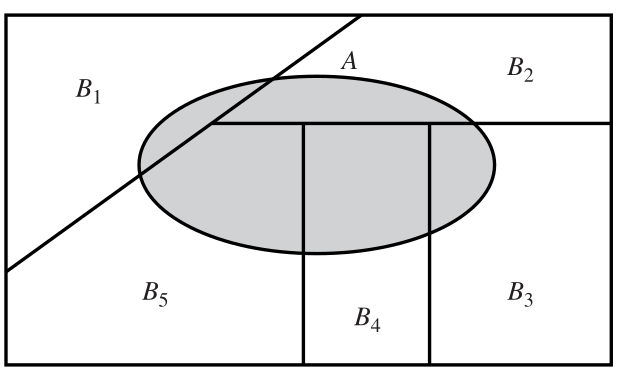
\includegraphics[scale = .4]{images/partition.png}
\end{center}
	
\end{figure}

It turns out that in this case we can write the probability of $A$ with the conditional probability of $\operatorname{P}\left(A | B_{j}\right)$ and $\operatorname{P}\left(B_{j}\right)$. Following theorem shows this

\begin{theorem}[Law of total probability]
	Suppose that the events $B_{1}, \ldots, B_{k}$ form a partition of the sample space $\Omega$ and $\operatorname{P}\left(B_{j}\right)>0$ for $j=1, \ldots, k .$ Then, for every event $A$ in $\Omega$

	\begin{align*}
		\operatorname{P}(A)=\sum_{j=1}^{k} \operatorname{P}\left(B_{j}\right) \operatorname{P}\left(A | B_{j}\right)
	\end{align*}


\end{theorem}

\section{Independent Events}

The conditional probability of the event $A$ given that the event $B$ has occurred is the revised probability of $A$ after we learn that $B$ has occurred. It might be the case, however, that no revision is necessary to the probability of $A$ even after we learn that $B$ occurs. In this case, we say that $A$ and $B$ are independent events. 


\begin{example}[Toss a coin and roll a dice togther]
If we toss a coin and then roll a die, we could let $A$ be the event that the die shows $3$ and let $B$ be the event that the coin lands with heads up. If the tossing of the coin is done in isolation of the rolling of the die, we might be quite comfortable assigning $\operatorname{P}(A | B)=\operatorname{P}(A)=1 / 6$. In this case, we say that $A$ and $B$ are independent events.
\end{example}

In general, if $\operatorname{Pr}(B)>0,$ the equation $\operatorname{P}(A | B)=\operatorname{P}(A)$ can be rewritten as $\operatorname{P}(A \cap B )/ \operatorname{P}(B)=\operatorname{P}(A)$. If we multiply both sides of this last equation by $\operatorname{P}(B),$ we obtain the equation $\operatorname{P}(A \cap B)=\operatorname{P}(A) \operatorname{P}(B) .$ In order to avoid the condition $\operatorname{P}(B)>0,$ the mathematical definition of the independence of two events is stated as follows:


\begin{definition}[Independent Events]
Two events $A$ and $B$ are independent if

\begin{align*}
	\operatorname{Pr}(A \cap B)=\operatorname{Pr}(A) \operatorname{Pr}(B)
\end{align*}

\end{definition}


Lets look at an example, 


\begin{example}
	Suppose that a fair coin is tossed twice. The experiment has four outcomes, HH, HT, TH, and TT, that tell us how the coin landed on each of the two tosses. We can assume that this sample space is simple so that each outcome has probability $1 / 4 .$ Suppose that we are interested in the second toss. In particular, we want to calculate the probability of the event $A=\{H \text { on second toss }\}$. We see that $A=$ $\{\mathrm{HH}, \mathrm{TH}\},$ so that $\operatorname{P}(A)=2 / 4=1 / 2 .$ If we learn that the first coin landed $\mathrm{T}$, we might wish to compute the conditional probability $\operatorname{P}(A | B)$ where $B=\{\text { T on first toss }\}$ Using the definition of conditional probability, we easily compute

	\begin{align*}
		\operatorname{P}(A | B)=\frac{\operatorname{P}(A \cap B)}{\operatorname{P}(B)}=\frac{1 / 4}{1 / 2}=\frac{1}{2}
	\end{align*}

	because $A \cap B=\{T H\}$ has probability $1 / 4 .$ We see that $\operatorname{P}(A | B)=\operatorname{P}(A) ;$ hence, we don't change the probability of $A$ even after we learn that $B$ has occurred.
\end{example}



\section{Indepdendence of several events}

The definition of independent events can be extended to any number of events, $A_{1} \ldots \ldots, A_{k} .$ Intuitively, if learning that some of these events do or do not occur does not change our probabilitics for any events that depend only on the remaining events, we would say that all $k$ events are independent.

















\appendix
\chapter{Appendix: Set Theory }

Sets are constantly encountered in mathematics. One speaks of sets of points, collections of real numbers, and families of functions. A set is conceived simply as a collection of definable and unique objects. The words set, collection, and family are all synonymous. The notation $x \in A$ means that $x$ is an element of the set $A$; the notation $x \notin A$ means that $x$ is not an element of the set $A$. A set can be described by listing its elements, usually within braces For
example,

\[
A=\{-1,2,5,4\}
\]

describes the set consisting of the numbers $-1,2,4,$ and $5 .$ More generally, a set $A$ may be defined as the collection of all elements $x$ in some larger collection satisfying a given property. Thus the notation

\[
A=\{x: P(x)\}
\]

defines $A$ to be the set of all objects $x$ having the property $P(x)$. This is usually read as "A equals the set of all elements $x$ such that $P(x)$." For example, if $x$ ranges over all real numbers, the set $A$ defined by

\[
A=\{x: 1<x<5\}
\]

is the set of all real numbers that lie between 1 and $5 .$ For this example, $3.75 \in A$ whereas $5 \notin A .$ We will also use the notation $A=\{x \in X: P(x)\}$ to indicate that only those $x$ that are elements of $X$ are being considered. Some basic sets that we will encounter throughout the text are the following:

$\mathbb{N}=$ the set of natural numbers or positive integers $=\{1,2,3, \ldots,\}$ \\
$\mathbb{Z}=\text { the set of all integers }=\{\ldots,-2,-1,0,1,2, \ldots,\}$\\
$Q=$ the set of rational numbers $=\{p / q: p, q \in \mathbb{Z}, q \neq 0\},$ \\
and $\mathbb{R}=$ the set of real numbers.


\textbf{\S. Using Venn diagrams for sets}

We will often use Venn diagrams to represent sets. Normally in a Venn diagram we draw sets using some objects like circles or squares and then show different relations between sets. 

\begin{definition}[Containment]
	It is said that a set $A$ is contained in another set $B$ if every element of the set $A$ also belongs to the set $B$. This relation between two set is expressed symbolically by the expression $A \subset B,$ which is the set-theoretic expression for saying that $A$ is a subset of $B$. Equivalently, if $A \subset B$, we may say that $B$ contains $A$ and may write $B \supset A$
\end{definition}

For containment, if $A \subset B$, we can draw this in a Venn diagram,


\begin{figure}[H]
	\begin{center}
		\begin{tikzpicture}

	    	\fill[gray!30!white]   (90:0) circle[radius=50pt] (2);
	    	\fill[white] (94:0) circle[radius=20pt] (2);
	    	% \draw (-2,-2) rectangle (3,2);

	  		\node at ( 90:0)    {$A$};
	  		\node at (94:1)    {$B$};
		\end{tikzpicture}
	\end{center}
\end{figure}




Now we can also probe can prove following theorem (try this!)

\begin{theorem}
Let $A, B,$ and $C$ be sets. If $A \subset B$ and $B \subset A,$ then $A=B .$ If $A \subset B$ and $B \subset C,$ then $A \subset C$
\end{theorem}

\begin{definition}
	The set contains no elements is called the empry set, or null set, and it is denoted by the symbol $\emptyset$. 
\end{definition}

Some sets contain only finitely many elements, while others have infinitely many elements. There are two sizes of infinite sets that we need to distinguish.


\begin{definition}[Countable/Uncountable.]
	 An infinite set $A$ is countable if there is a one-to-one corrspondence between the elements of $A$ and the set of natural numbers $(1,2,3, \ldots)$. A set is uncountable if it is neither finite nor countable. If we say that a set has at most countably many elements, we mean that the set is either finite or countable.
\end{definition}
 
\begin{definition}[Empty set]

A set which has no elements is called an empty set and we denote this with $\emptyset$
	
\end{definition}

Note if you take any set $A$, then $\emptyset \subset A$. This might look strange. But this is true because empty set has nothing if include all the elements of the empty set we include nothing. Also another important point any set $A \subset A$.

\begin{definition}[Power set]
If $A$ is a set, the set of all subsets of $A$ is called the power set of $A$ and we denote this with $\mathscr{P}(A)$.
\end{definition}

\begin{example}[example of a power set]
If $A=\{1,2\},$ then

\begin{align*}
	\mathscr{P}(A)=\{\phi,\{1\},\{2\},\{1,2\}\}
\end{align*}


\end{example}

In the last example, the set $A$ has 2 elements and $\mathscr{P}(A)$ has 4 or $2^{2}$ elements, the elements in this instance being the subsets of $A$. If we take a set with 3 elements, then by listing the subsets of $A$ it is easily seen that there are exactly $2^{3}$ subsets of $A$ (Exercise 8 ). On the basis of these two examples we are inclined to conjecture that if $A$ contains $n$ elements, then $\mathscr{P}(A)$ contains $2^{n}$ elements. Note in the example we also included $\emptyset$ and the whole set $A$ as well.

\section{Operations on sets}

Now we come to certain operations on sets. Here we will need a special concept, that we call universal set. A universal set is just like a set. But the idea is whenever we have an universal set. All the other sets are subsets of the universal set. Often its denoted with $U$


\begin{definition}[Complement]
The complement of a set $A$ with respected to the universal set $A$ is defined to be the set that contains all elements of $U$ that do not belong to $A .$ The notation for the complement of $A$ is $A^{c}$. 


\end{definition}

Note the concept complement needs a universal set, otherwise it does not make it sense. Here is the Venn diagram of $A^c$.

\begin{figure}[H]
	\begin{center}
		\begin{tikzpicture}

	    	%\fill[white] (94:0) circle[radius=20pt] (2);
	    	\fill[gray!30!white] (-2,-2) rectangle (3,2);
	    	\fill[white]   (90:0) circle[radius=50pt] (2);


	  		%\node at ( 90:0)    {$A$};
	  		\node at (94:1)    {$A$};
	  		\node at (130:2.3)    {$U$};
		\end{tikzpicture}
	\end{center}
\end{figure}

following are the events,


\begin{figure}[H]
\begin{venndiagram2sets}
\fillA \fillB
\end{venndiagram2sets}%
\begin{venndiagram2sets}
\fillACapB
\end{venndiagram2sets}
\caption{Left: $A\cup B$ and right $A\cap B$}
\end{figure}





\end{document}